\chapter{State of the art}
\label{ch:stateoftheart}

This chapter gives an overview of previous work, and how this thesis fits within those studies.

\section{Smart cities}

In the last few years, smart cities have been a hot topic in research \cite{caragliu_bo_nijkamp_2011} given the quantity of available data provided by the internet of things \cite{zanella_bui_castellani_vangelista_zorzi_2014} and big data \cite{townsend_2013} and the newest infrastructures that allow cities to track activities in real time. This leads to the use of this data to improve the quality of life of the citizen, employment\cite{shapiro_2005},saving on unused services when they are not necessary and limiting the pollution by making smart transport more fluid.

Some cities are already taking advantage of this technology \cite{wikipedia_smart_cities}, Amsterdam already monitors traffic in real time and shows information about the best route to take, Barcelona has already optimized bus routes through the center to optimize the number of green lights they encounter.

Smart cities also monitor pedestrian activities to know when to dim lights on the night, or when to put a traffic light green if no one is getting to that intersection. The main concern of a smart city is to save energy, and make the quality of their citizens life as good as possible.

Smart cities is a general idea of which smart transport is only a small part, this thesis focuses on that part, trying to minimize the time spent on the road and thus, the generated pollution.

\section{Smart transport}

Smart transport is a topic that only recently has started to be researched. \cite{lenior_janssen_neerincx_schreibers_2006} defines Smart transport as \glqq adequate human–system symbiosis to realize effective, efficient and human-friendly transport of goods and information.\grqq, I would add that smart transport also focuses on minimizing pollution and that is exactly what this thesis is focusing on, a protocol that will make transportation effective, efficient and greener while being human-friendly.

As seen in this review \cite{perez_carrillo_montoya-torres_2014} the criteria to find the best protocol is very varied, it can be based on  social, economic, environmental or even land usage. Our protocol is focused on minimize the network congestion and thus minimizing the total added time of travel times.

This MAS helps analysts to test different routing algorithms in a distributed way, and mix different algorithms within the same simulation. I believe that this tool will be really useful for anyone that wants an initial test since its usage and output are so easily learned. 

\section{Routing algorithms}
\label{algorithms}

In this chapter, well known routing algorithms are proposed and studied.

\subsection{What is a routing algorithm}

A routing algorithm is a deterministic program that finds a path between an origin and a destination. Usually the network where the path has to be extracted from is a graph, directed or undirected.

A basic graph has two main components, vertices and edges. In the context of this thesis, the vertices are traffic intersections and the edges are the roads that connect them.

Edges usually come with a weight, it is a value that represents the cost of traversing that edge, this could be anything from kilometers to time. Graphs can even have more than one kind of weight depending on what we intend to optimize.

In the context of this thesis, the roads have their length and the maximum allowed speed, this allows us to use the most simple metrics on traffic, time and distance.

A routing algorithm takes advantage of all this information and finds the minimum path depending on the metric we want to optimize, in our case time or distance.

In this thesis we are going to focus on the most simple yet effective path finding algorithms.

\subsubsection{Dijkstra's algorithm}

% Estado del arte sobre el algoritmo de dijkstra

Dijskstra's algorithm is a well known iterative algorithm that finds the shortest path between two nodes in its most simple version. This is the most famous path finding algorithm and has been deeply studied \cite{dijkstra_1} \cite{dijkstra_2}.

Its pseudocode is the following:

\begin{figure}[!ht]
  \centering
  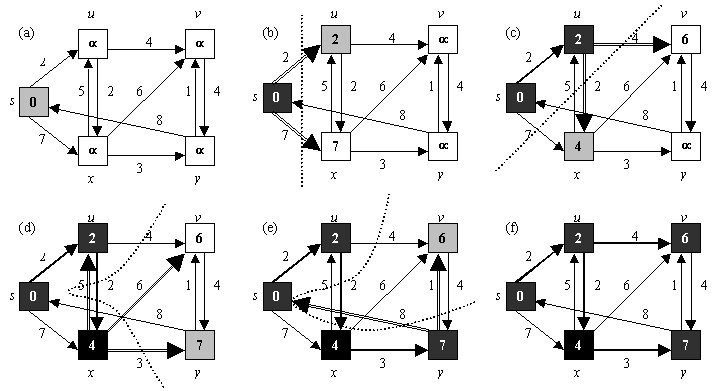
\includegraphics[scale=0.5]{images/dijkstra.jpg} 
  \caption{Dijkstra's algorithm path finding}
  \label{dijkstra}
\end{figure}

As an example of how it finds the optimal path, let's use graph \ref{dijkstra}\footnote{Image from \url{http://cs.smith.edu/~streinu/Teaching/Courses/274/Spring98/Projects/Philip/fp/dijkstra.htm}}, the value inside the boxes is the distance that takes to go from the initial node (in this case the initial node is $s$) to each node. As seen in the pseudocode, all node values have been set to infinity except the departure node.

Nodes in gray represent the node that we are examining, nodes in black are those whose minimum distance has already been found, and the dotted line represents a virtual delimiter for the nodes whose distance has already been determined.

To find the shortest path from $s$ to $v$, we start at $s$, since it has the minimum distance of all the nodes, and draw the virtual dotted line between it and the rest of the nodes (a and b). We now evaluate the vertex that are cut with that line, the lengths are 2 (between $s$ and $u$) and 7 (between $s$ and $x$). We now have evaluated the node $u$, so we update the position of the dotted line. We now consider all the nodes that cur that line and have not been considered yet, that cut gives us the values 4 (between $u$ and $v$) and 6 (between $x$ and $v$), since the minimum added distance from $s$ to $v$ (going through $u$) is less than infinity, we update its distance (c).

We keep this process until all distances have been found, or we can stop when the desired distance between the origin node and the destination node is found.

\begin{verbatim}
function Dijkstra(Graph, source):

    for each vertex v in Graph:	// Initialization
        dist[v] := infinity	// initial distance from source to vertex v 
                            //is set to infinite
        previous[v] := undefined	// Previous node in optimal path from source
        
    dist[source] := 0	// Distance from source to source
    
    Q := the set of all nodes in Graph	// all nodes in the graph
                                        //are unoptimized - thus are in Q
    
    while Q is not empty:	// main loop
        u := node in Q with smallest dist[ ]
        remove u from Q
        
        for each neighbor v of u:	// where v has not yet been removed from Q.
            alt := dist[u] + dist_between(u, v)
            
            if alt < dist[v]	// Relax (u,v)
                dist[v] := alt
                previous[v] := u
                
return previous[]
\end{verbatim}

\subsubsection{Bellman-Ford algorithm}

Dijkstra's algorithm has a weakness with negative cycles, for example the solution for the graph in Figure \ref{unsolvable}, will not be the optimal, since the distance between $A$ and $C$ found by Dijkstra's will be 0 instead of the minimum of -200.

Bellman-Ford's algorithm is a well known variation of Dijkstra's algorithm that is able to solve graphs with in which some of the edges are negatives, as long as there is not a negative cycle. It is slower than Dijkstra's algorithm for the same problem but it is more versatile.

\begin{figure}[!ht]
  \centering
  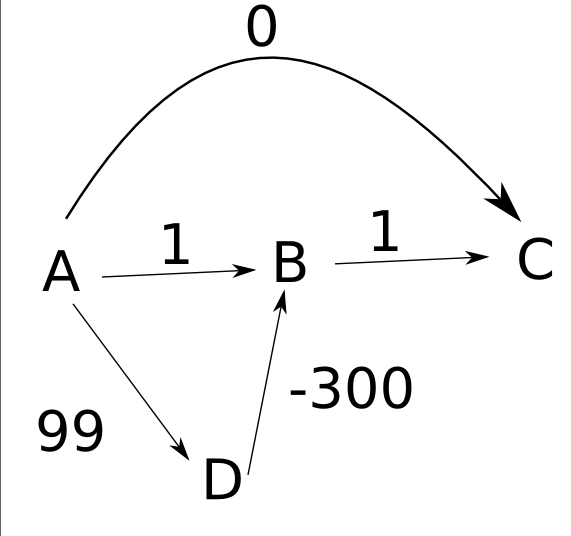
\includegraphics[scale=0.2]{images/rmowk.png} 
  \caption{An unsolvable graph for Dijkstra}
  \label{unsolvable}
\end{figure}

Its pseudocode is the following:

\begin{verbatim}
 function BellmanFord(list vertices, list edges, vertex source)
   ::distance[],predecessor[]

   // This implementation takes in a graph, represented as
   // lists of vertices and edges, and fills two arrays
   // (distance and predecessor) with shortest-path
   // (less cost/distance/metric) information

   // Step 1: initialize graph
   for each vertex v in vertices:
       distance[v] := inf             // At the beginning , all vertices 
                                      //have a weight of infinity
       predecessor[v] := null         // And a null predecessor
   
   distance[source] := 0              // Except for the Source, 
                                      //where the Weight is zero 
   
   // Step 2: relax edges repeatedly
   for i from 1 to size(vertices)-1:
       for each edge (u, v) with weight w in edges:
           if distance[u] + w < distance[v]:
               distance[v] := distance[u] + w
               predecessor[v] := u

   // Step 3: check for negative-weight cycles
   for each edge (u, v) with weight w in edges:
       if distance[u] + w < distance[v]:
           error "Graph contains a negative-weight cycle"
   return distance[], predecessor[]
\end{verbatim}

Given that there are not negative weights in our road network and that given the same graph, Bellman-Ford's takes longer than Dijkstra, this algorithm is not preferred to Dijkstra.

\subsubsection{A* algorithm}

A* is a variation of Dijkstra's algorithm widely used for pathfinding in videogames. Actually Dijsktra's algorithm is a special case of A*, when the heuristics are zero. 

%It uses a heuristic to estimate if the node to study looks promising, cutting the complexity time. This algorithm heavily relies on the heuristic function and does not guarantee the optimal path, that's why this algorithm has not been chosen.

Its pseudocode is the following:

\begin{verbatim}
function A*(start, goal)
    // The set of nodes already evaluated.
    closedSet := {}
    // The set of currently discovered nodes still to be evaluated.
    // Initially, only the start node is known.
    openSet := {start}
    // For each node, which node it can most efficiently be reached from.
    // If a node can be reached from many nodes, cameFrom will eventually 
   	//contain the
    // most efficient previous step.
    cameFrom := the empty map

    // For each node, the cost of getting from the start node to that node.
    gScore := map with default value of Infinity
    // The cost of going from start to start is zero.
    gScore[start] := 0 
    // For each node, the total cost of getting from the start node to the goal
    // by passing by that node. That value is partly known, partly heuristic.
    fScore := map with default value of Infinity
    // For the first node, that value is completely heuristic.
    fScore[start] := heuristic_cost_estimate(start, goal)

    while openSet is not empty
        current := the node in openSet having the lowest fScore[] value
        if current = goal
            return reconstruct_path(cameFrom, current)

        openSet.Remove(current)
        closedSet.Add(current)
        for each neighbor of current
            if neighbor in closedSet
                continue		// Ignore the neighbor which is already evaluated.
            // The distance from start to a neighbor
            tentative_gScore := gScore[current] + dist_between(current, neighbor)
            if neighbor not in openSet	// Discover a new node
                openSet.Add(neighbor)
            else if tentative_gScore >= gScore[neighbor]
                continue		// This is not a better path.

            // This path is the best until now. Record it!
            cameFrom[neighbor] := current
            gScore[neighbor] := tentative_gScore
            fScore[neighbor] := gScore[neighbor] +
                                heuristic_cost_estimate(neighbor, goal)

    return failure

function reconstruct_path(cameFrom, current)
    total_path := [current]
    while current in cameFrom.Keys:
        current := cameFrom[current]
        total_path.append(current)
    return total_path
\end{verbatim}

% Comparativa entre entre el A* y Ddijkstra

The main difference between A* and Dijsktra is that A* is an informed version of Dijkstra, where using the heuristic a priority can be set to chose one node over the other. It makes the pathfinding faster, but since getting a good heuristic requires a detailed study of the system, Dijkstra was chosen over A*,

\subsection{Chosen algorithms}

As detailed in the previous section, the most common algorithms have been studied to find the one that better fits the system. Each one has its benefits, but in the end Dijkstra's algorithm has been chosen due to its ease of use and modification.

\subsubsection{Shortest path algorithm}

The shortest path algorithm used in this simulator is the most basic implementation of Dijkstra's, knowing the distance between all the intersections the car finds its path looking for the one that takes less distance for it.

This method is deterministic, any car wanting to go from point A to point B will have the same path. Given the dynamic nature of the traffic, this will lead to significant traffic jams if the chosen path crosses a segment that congests very easily.

\subsubsection{Fastest path algorithm}

The fastest path algorithm is a slight modification of the previous algorithm, it only differs on searching for the minimum time instead of the minimum distance.

For each segment the maximum speed a car can drive on it is \[Speed_{max} = min(\text{max speed on that segment} | \text{max speed of the car})\]

Because the maximum speed of each car is different, different paths from A to B can be found, which makes this algorithm slightly better to avoid traffic jams. However, it does so by accident and many cars will chose the same path.

\subsubsection{Smart path algorithm}

The smart path algorithm takes into account the state of the traffic in real time and avoids congested paths. This is the proposed algorithm and it is expected to behave much better than the others.

Again, this algorithm is a modification of Dijkstra's algorithm that minimizes the time that takes the car from going to point A to B. This algorithm is very similar to the previous one, but it takes into account the \emph{current} maximum speed of that segment such that

\[Speed_{max} = min(\text{current max speed on that segment} | \text{max speed of the car})\]

so if a segment is congested the car simply avoids it. Because segments are dynamically congested, this algorithm recalculates its path at every intersection, given that you cannot turn around inside a segment this algorithm effectively keeps you in the fastest path at every moment.


% Seccion de Design and Implementation: 
% Grafico con la estructura interna del programa
% Detalles sobre la implementación que posdrían ser interesantes, optimizaciones, ficheros de configuración, etc.
% Algunas dificultades interesantes -> JADE no funcionaba bien.

% Section Test and Results
% Explicar test, escenario del test
% Explicar resultados

% Section Conclusion
% Achivment of objectivs: comentas los resultados obtenidos
% Aplicación de los conocimientos adquiridos en el master
% Future work
% Personal Evaluation





